\documentclass{article}
\usepackage[utf8]{inputenc}

\title{Quantum Mechanics and Path Integrals Selected Book Solutions (R.P. Feynman and A.R. Hibbs) }
\author{jaderosenblitt }
\date{January 2021}

\usepackage{amsmath}
\usepackage{physics}
\usepackage{natbib}
\usepackage{graphicx}
\usepackage{parskip} %this helps disable paragraph indenting

\begin{document}

\maketitle

\section{Introduction}
There is a theory which states that if ever anyone discovers exactly what the Universe is for and why it is here, it will instantly disappear and be replaced by something even more bizarre and inexplicable.
There is another theory which states that this has already happened.

\subsection{Probability in Quantum Mechanics}

%I am writing a physics equations. 
%
%\begin{equation}
%    \bra{h} = \frac{1}{2}\bra{c}
%\end{equation}

%\begin{figure}[h!]
%\centering
%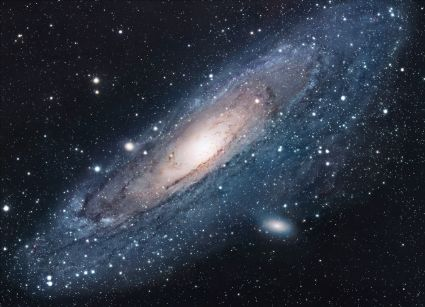
\includegraphics[scale=1.7]{universe}
%\caption{The Universe}
%\label{fig:universe}
%\end{figure}

%Section 2
\section{The Quantum Mechanical Law of Motion}

\subsection{The Classical Action}

\textbf{Problem 2-1}
For a free particle $L = (m/2)\dot{x}^2$. Show that the action $S_{cl}$ corresponding to the classical motion of a free particle is 

$S_{cl} = \frac{m}{2}\frac{(x_{b} - x_{a})^2}{(t_{b} - t_{a})}$



\textbf{Solution:} 

Since $L$ is given by 

\begin{align*}
         L = \frac{m}{2}\dot{x}^2
\end{align*}

we use the Euler-Lagrange equation, 

\begin{align*}
         \pdv{L}{x} - \frac{d}{dt}\Big( \pdv{L}{\dot{x}} \Big) = 0
\end{align*}

we first calculate using $L$ the partial derivative $\pdv{L}{x}$, 

\begin{align*}
    \pdv{L}{x} = 0
\end{align*}

because $L$ does not depend on $x$ explicitly. Next we find $\pdv{L}{\dot{x}}$:

\begin{align*}
         \pdv{L}{\dot{x}} = \frac{2}{2}m\dot{x} = m\dot{x}
\end{align*}

next we take the derivative with respect to $t$ which gives 

\begin{align*}
         \frac{d}{dt}\Big( \pdv{L}{\dot{x}} \Big) = m\frac{d}{dt}(\dot{x}) = m\frac{d^{2}x}{dt^{2}} = m\Ddot{x}
\end{align*}

Plugging both equations above into out Euler Lagrange equation simply gives  

\begin{align*}
         0 - m\frac{d^{2}x}{dt^{2}} = 0
\end{align*}

so that after dividing by $-m$ we are left with the simple second-order ordinary differential equation 

\begin{align*}
         \frac{d^{2}x}{dt^{2}} = 0
\end{align*}

In physical terms, all this equation is saying is that the acceleration is $0$. Therefore, if there is no acceleration, the particle is moving with a constant velocity, in other words, $\dot{x} = const$, in which case we can just set $\dot{x}$ to be the average velocity,

\begin{align*}
    \dot{x} = \frac{x(t_{b}) - x(t_{a})}{t_{b} - t_{a}}
\end{align*}

Therefore, to find $S_{cl}$, we must use 

\begin{align*}
    S_{cl} = \int_{t_{a}}^{t_{b}} L(x,\dot{x},t) dt
\end{align*}

and so 

\begin{align*}
    S_{cl} = \int_{t_{a}}^{t_{b}} L(x,\dot{x},t) dt = \int_{t_{a}}^{t_{b}} \frac{m}{2}\dot{x}^2 dt = \frac{m}{2}\dot{x}^2\int_{t_{a}}^{t_{b}} dt
\end{align*}

where the inside term containing $\dot{x}$ and all constants were brought outside because as just discussed, $\dot{x}$ is itself a constant (constant velocity). Plugging in our previous equation obtained and doing the integral just gives 

\begin{align*}
    S_{cl} = \frac{m}{2}\dot{x}^2\int_{t_{a}}^{t_{b}} dt = \frac{m}{2}\Big( \frac{x(t_{b}) - x(t_{a})}{t_{b} - t_{a}} \Big)^{2} (t_{b} - t_{a}) = \frac{m}{2}\frac{(x(t_{b}) - x(t_{a}))^{2} }{t_{b} - t_{a}}
\end{align*}

where the square term at the bottom was reduced by one power because of the time difference at the top that resulted from the integral. 

Alternatively integration by parts can be used in the second last step but we will not demonstrate it here. The reader is encouraged to try it for themselves if they feel so inclined. However, it does not appear to provide much new insight, if any, that the author is aware of currently. 

\subsection{The Quantum-Mechanical Amplitude}

\subsection{The Classical Limit}

% \begin{figure}[!p]
% 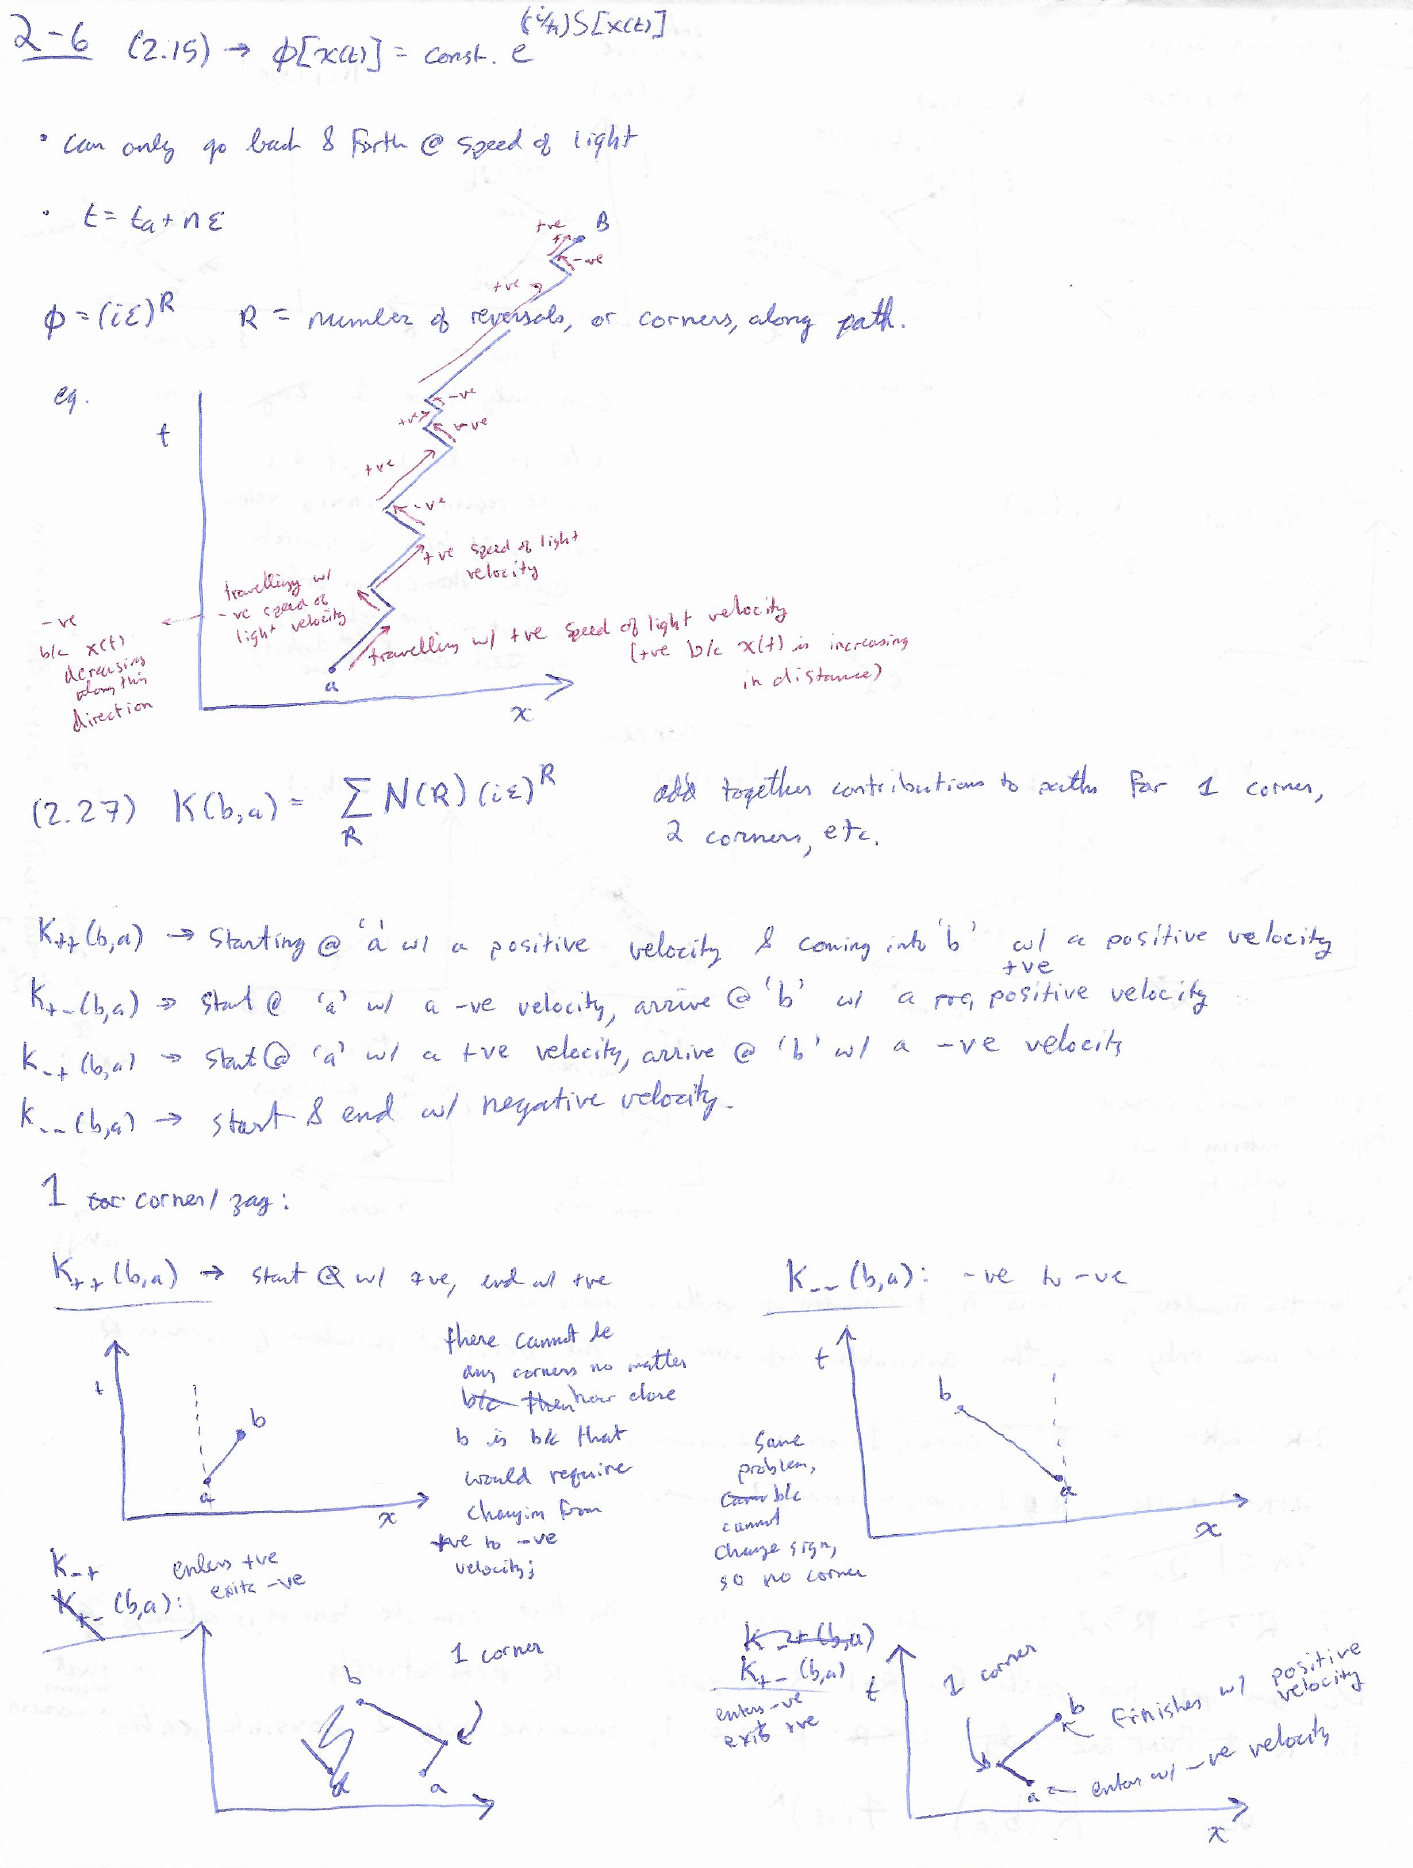
\includegraphics[width=15cm]{FeynmanQ2dash6p1.png}
% \end{figure}


\subsection{The sum over paths}
\textbf{Question 2-6} Refer to the solutions given by images at the end of this document 


\section{Developing the Concepts with Special Examples}
\subsection{This is a }


\section{The Schrodinger Description of Quantum Mechanics}

\subsection{The Schrodinger Equation}
\textbf{Question 4-3} Show that the complex conjugate function $\psi^{*}$ (all $i$'s changed to $-i$'s) satisfies 
\begin{equation*}
    \pdv{\psi^{*}}{t} = +\frac{i}{\hbar}(H\psi)^{*}
\end{equation*}

\textbf{Solution:}
Using (4.14), 
\begin{equation*}
    \pdv{\psi}{t} = - \frac{i}{\hbar}H\psi
\end{equation*}
and taking the complex conjugate of both sides yields 

\begin{equation*}
    \Big( \pdv{\psi}{t} \Big)^{*} = \Big( - \frac{i}{\hbar}H\psi \Big)^{*} \Leftrightarrow  \pdv{\psi^{*}}{t} = +\frac{i}{\hbar}(H\psi)^{*}
\end{equation*}

\textbf{Question 4-4} Show 
\begin{equation*}
    \pdv[2]{}{x}x = x\pdv[2]{}{x} + 2 \pdv{}{x} 
\end{equation*}
\textbf{Solution:} 

\noindent Hint: (4.21) (below) is very helpful. 
\begin{equation*}
    \pdv{}{x}x = x\pdv{}{x} + 1
\end{equation*}

\noindent Full solution: 

\begin{multline*}
     \pdv[2]{}{x}x = \pdv{}{x} \Bigg( \pdv{}{x}x \Bigg) = \pdv{}{x} \Bigg( x\pdv{}{x} + 1 \Bigg) = \pdv{}{x} \Bigg( x\pdv{}{x} \Bigg) + \pdv{}{x} \\ = x \pdv[2]{}{x} + (1)\pdv{}{x} + \pdv{}{x} =  x\pdv[2]{}{x} + 2 \pdv{}{x}   
\end{multline*}
where the distributive property was used in the third step and the product rule in the fourth. 

To answer the second part, just write out the full form of H using (4.15) and insert that into the left side of (4.23) then use the newly proven (4.22) to simplify the equation to the right hand side of (4.23) 

Note here that $H = \frac{-\hbar^{2}}{2m}\pdv[2]{}{x} + V(x,t)$. Thus, 

\begin{align*}
    Hx -xH  &=\frac{-\hbar^{2}}{2m}\pdv[2]{}{x}x + V(x,t)x - x\frac{-\hbar^{2}}{2m}\pdv[2]{}{x} - xV(x,t) \\
     &=\frac{-\hbar^{2}}{2m}\Bigg( x\pdv[2]{}{x} + 2 \pdv{}{x} \Bigg) + V(x,t)x - x\frac{-\hbar^{2}}{2m}\pdv[2]{}{x} - xV(x,t) \\
      &=\frac{-\hbar^{2}}{2m}2\pdv{}{x} \\
      &= \frac{-\hbar^{2}}{m}\pdv{}{x}
\end{align*}

where we have assumed that $[V(x,t),x]=0$

\textbf{Bonus}:
What about $\pdv[3]{}{x}x$? We use the result above obtained for the case  $\pdv[2]{}{x}x$.

\begin{align*}
    \pdv[3]{}{x}x  &=\pdv{}{x} \Bigg( \pdv[2]{}{x}x \Bigg) \\
     &=\pdv{}{x} \Bigg( x\pdv[2]{}{x} + 2\pdv{}{x}  \Bigg) \\
      &=\pdv{}{x}\big( x\pdv[2]{}{x} \big) + 2\pdv{}{x}\big( \pdv[]{}{x} \big)  \\
      &= x\pdv[3]{}{x} + (1)\pdv[2]{}{x} + 2\pdv[2]{}{x}   \\
      &= x\pdv[3]{}{x} + 3\pdv[2]{}{x}
\end{align*}

where the product rule was used to obtain the fourth line. One can conjecture and probably prove the operator formula 

\begin{align*}
    \big( \pdv[n]{}{x} \big) x  &=x\pdv[n]{}{x} + n\pdv[n-1]{}{x}
\end{align*}

where $n$ refers to the $n$-th derivative wrt $x$, or in proper operator notation using $D_{x}$ to stand for the differentiation operator with respect to $x$, 

\begin{align*}
    D_{x}^{n} x  &=xD_{x}^{n} + nD_{x}^{n-1}
\end{align*}

where again we emphasize that on the left hand side, since these are operators, we have the operator that applies the $n$-th derivative \textit{multiplying} the operator that takes some state/function/etc $\psi$ and multiplies it by x. The operator $D_{x}$ is \textit{not} acting on $x$. If $\psi$ is, for example, some function of $x$ and we call the operator $M_{x}$ the operator that multiplies something by $x$ (for example, $M_{x} \psi(x) = x\psi (x)$), then we get using the same notation as before for the operator equation on $\psi$ as 

\begin{align*}
        \big( D_{x}^{n} M_{x} \big) \psi (x)  &=\big( M_{x}D_{x}^{n} + nD_{x}^{n-1} \big) \psi (x)
\end{align*}

The relation can be simply be summarized as 

\begin{align*}
        [D_{x}^{n}, M_{x}]  &= nD_{x}^{n-1}
\end{align*}

where again the square brackets refer to the commutator, ie $[x,y] = xy - yx$. 

Although this is one case, let's take a look at what happens if we switch the roles and instead of modifying the derivative operator, we change the multiplication operator to be "multiply by $x^2$" instead of $x$. 

As Feynman originally presented on page 80, let's modify his approach and let $A$ be the operator that takes the first derivative, ie $A = D_{x} = \pdv{}{x}$ and $B$ is the opertor that multiplies by $x^2$. 

We first need to modify Feynman's result, ie that $\pdv{}{x} \big(x\psi\big) = x\pdv{\psi}{x} + \psi$. Since we now instead multiply by $x^2$, the result becomes: 

\begin{align*}
        \pdv{}{x} \big(x^{2}\psi\big) &= x^{2}\pdv{\psi}{x} + 2x\psi
\end{align*}

Using this, similar to Problem 4-4, we ask the following: 

\textbf{Problem: Bonus}
$A^{2}B =  \pdv[2]{}{x} x^{2} = ?$

Solution: 

\begin{align*}
     \pdv[2]{}{x}x^{2} &=\pdv{}{x} \Bigg( \pdv[]{}{x}x^{2}  \Bigg) \\
     &=\pdv{}{x} \Bigg( x^{2}\pdv{}{x} + 2x \Bigg) \\
      &=\pdv{}{x} \big( x^{2}\pdv{}{x} \big)  + 2\pdv{}{x}x\\
      &= x^{2}\pdv[2]{}{x} + 2x\pdv{}{x} + 2\pdv{}{x}x  
\end{align*}

while it may not look obvious at first, re-writing this in the differential operator notation proper gives the relation:

\begin{align*}
        \big( D_{x}^{2} M_{x^{2}} \big) &=\big( M_{x^{2}}\big( D_{x}^{2} \big) + 2M_{x}\big( D_{x} \big) + 2\big( D_{x} \big)M_{x} \big) 
\end{align*}

(where $M_{x^{2}}$ refers to the operator that multiplies by $x^2$) but after factoring out the 2 and moving the first term on the right hand side to the left, we obtain 

\begin{align*}
         D_{x}^{2} M_{x^{2}} - M_{x^{2}}\big( D_{x}^{2} \big)  &=2\big( M_{x}\big( D_{x} \big) + \big( D_{x} \big)M_{x} \big) 
\end{align*}

but looking closely, on the left we just have the commutator and on the right we have the well-known \textit{poisson brackets} or \textit{anticommutator} ie $\{a,b \} = ab + ba$. Thus we may re-write the operator equation as 

\begin{align*}
         [D_{x}^{2}, M_{x^{2}}] &=2\{M_{x},  D_{x} \}
\end{align*}

or 

\begin{align*}
         [D_{x}^{2}, M_{x^{2}}] &=2\{ D_{x}, M_{x} \}
\end{align*}


since we have assumed commutativity in the addition of the operators, ie that $AB + BA = BA + AB$. 

Further interesting properties may be derived from this point, either by looking at an operator that multiplies by the $n$-th power of the variable or mixing the number of derivatives and the powers. Actually, this relation speaks to a deeper aspect of both the differentiation operator and the multiplication operator. A good starting guide can be found in section 10.7 of Kreyszig's "Introductory Functional Analysis with Applications" and Helmberg's "Introduction to Spectral Theory in Hilbert Space" Chapter IV, Section 18.\citep{kreyszigfunctional} Due to the author's laziness, he leaves it to the reader to try it for themselves using this question as a starting point. 

% \begin{align}
%     B' &=-\nabla \times E,\\
%     E' &=\nabla \times B - 4\pi j
% \end{align}


\textbf{Question 4-5} Using the relation 
\begin{equation*}
    K(b,a) = \int_{-\infty}^{\infty} K(b,c)K(c,a) dx_{c}
\end{equation*}
with $t_{c} - t_{a} = \epsilon$, an infinitesimal, show that if $t_{b} > t_{a} $ the kernel $K$ satisfies

\begin{equation*}
    \pdv{}{t_{a}} = K(b,a) = +\frac{i}{\hbar}H_{a}^{*}K(b,a) 
\end{equation*}

\textbf{Solution:} 

Hints: 

\begin{enumerate}
    \item $K(c,a) = K^{*}(a,c)$ (where $K^{*}$ is the complex conjugate)
    \item $[\pdv{}{t_{a}}, K(b,c)] = 0$ (i.e. they commute since it's independent of $a$ and $[ ]$ is the commutator, $[x,y] = xy - yx$)
    \item Following (4.21), \\ 
    if $\pdv{\psi ^{*}}{t} = +\frac{i}{\hbar}(H_{a}\psi)^{*}$ then $\pdv{}{t_{a}}K^{*}(a,c) = +\frac{i}{\hbar}\Big(H_{a}K(a,c)\Big)^{*} $
\end{enumerate}
    
Full Solution: 

\begin{multline*}
    K(b,a) = \int_{-\infty}^{\infty} K(b,c)K(c,a) dx_{c} \Longleftrightarrow \\ \pdv{}{t_{a}} K(b,a) =  \pdv{}{t_{a}} \int_{-\infty}^{\infty} K(b,c)K(c,a) dx_{c}
\end{multline*}
bringing the partial derivative inside and using hints 1 and 2 we have

\begin{equation*}
    \pdv{}{t_{a}} K(b,a) = \int_{-\infty}^{\infty} K(b,c) \pdv{}{t_{a}} K^{*}(a,c) dx_{c}
\end{equation*}
so that using hint 3 yields
 
\begin{equation*}
    \pdv{}{t_{a}} K(b,a) = \int_{-\infty}^{\infty} K(b,c) \Big( \frac{i}{\hbar}\Big(H_{a}K(a,c)\Big)^{*} \Big) dx_{c}
\end{equation*}
and applying the complex conjugate operator gives 

\begin{multline*}
    \pdv{}{t_{a}} K(b,a) = \int_{-\infty}^{\infty} K(b,c) \Big(  \frac{i}{\hbar} K^{*}(a,c)H_{a}^{*} \Big) dx_{c} \\ = \frac{i}{\hbar} H_{a}^{*} \int_{-\infty}^{\infty} K(b,c) K(c,a) dx_{c} = \frac{i}{\hbar} H_{a}^{*} K(b,a)
\end{multline*}
where constants have been taken out of the integral (i.e. $i, \hbar$), $H_{a}^{*}$ has been taken out since it is independent of the integration variable (recall (4.24)) and hint 1 has been used but to go back to the original kernel $K$. 

\textbf{Question 4-7} Show that $\int K^{*}(b,a)K(b,c)dx_{b} = K^{*}(c,a)$ with the usual $t_{b} > t_{c} > t_{a}$ convention holding.

\textbf{Solution:} 

Using (4.38), 
\begin{equation*}
    \int_{-\infty}^{\infty} K^{*}(b,c)K(b,a) dx_{b} = K(c,a)
\end{equation*}
we take the complex conjugate of both sides such that 
\begin{multline*}
    \Big( \int_{-\infty}^{\infty} K^{*}(b,c)K(b,a) dx_{b} \Big)^{*} = \Big( K(c,a) \Big)^{*} \\ 
    \Longleftrightarrow \int_{-\infty}^{\infty} ((K(b,a))^{*} (K^{*}(b,c))^{*} dx_{b} = K^{*}(c,a) \\
    \Longleftrightarrow \int_{-\infty}^{\infty} K^{*}(b,a)K(b,c) dx_{b} = K^{*}(c,a)
\end{multline*}
where the complex conjugate of the complex conjugate is the kernel itself. 


%\Longleftrightarrow


\section{Measurements and Operators}

\subsection{Measurement of quantum mechanical variables}

\textbf{Problem 5-3}
Assume $\int_{-\infty}^{\infty}f^{*}(x)f(x)dx$, which is the probability that a particle of wave function $f(x)$ is somewhere, has been normalized to the value 1. Under this constraint, show that the state $f(x)$ which has the highest probability of having the property $G$ is $f(x) = g(x)$

\textbf{Solution:} 
Note that if $f(x) = g(x)$, then $f^{*}(x) = g^{*}(x)$, where $*$ denotes the complex conjugate. Then the probability of having some property $\xi$ is 

\begin{align*}
         P(\xi) &= \bigg | \int_{-\infty}^{\infty}f^{*}(x)f(x)dx \bigg |^{2}
\end{align*}

using (5.32), 

\begin{align*}
         P(G) &= \bigg | \int_{-\infty}^{\infty}g^{*}(x)f(x)dx \bigg |^{2}
\end{align*}

where $g^{*}(x)$ is probability of having property $G$ but since $f^{*}(x) = g^{*}(x)$

\begin{align*}
         P(G) &= \bigg | \int_{-\infty}^{\infty}f^{*}(x)f(x)dx \bigg |^{2}
\end{align*}
 
which occurs when $f(x) = g(x)$.

\textbf{Problem 5-4}
Suppose the wave function for a system is $\psi (x)$ at time $t_{a}$. Suppose further that the behaviour of the system id described by the kernel $K(x_{b}, t_{b}; x_{a}, t_{a})$ for motions in the interval $t_{b} \geq t \geq t_{a}$. Show that the probability that the system is found to be in the state $\chi (x)$ at time $t_{b}$ is given by the square of the integral 

$\int_{-\infty}^{\infty}\int_{-\infty}^{\infty}\chi^{*}(x_{b})K(x_{b}, t_{b}; x_{a}, t_{a})\psi (x_{a})dx_{a}dx_{b}$

We call this integral the \textit{transition amplitude} to go from state $\psi(x)$ to state $\chi (x)$ 

\textbf{Solution:} 
We use (5.32), ie 

\begin{align*}
         P(G) &= \bigg | \int_{-\infty}^{\infty}g^{*}(x)f(x)dx \bigg |^{2}
\end{align*}

and identify that $g^{*}(x)$ is $\int_{-\infty}^{\infty}\chi^{*}(x_{b})dx_{b}$ and $f(x)$ is $\int_{-\infty}^{\infty}K(x_{b}, t_{b}; x_{a}, t_{a})\psi (x_{a})dx_{a}$. In other words, 

\begin{align*}
         P(\chi^{*}(x_{b})) &= \bigg | \int_{-\infty}^{\infty}\int_{-\infty}^{\infty}\chi^{*}(x_{b})K(x_{b}, t_{b}; x_{a}, t_{a})\psi (x_{a})dx_{a}dx_{b} \bigg |^{2}
\end{align*}
 


\subsection{}

\subsection{Operators}

\textbf{Problem 5-8} Note that equation (5.44) implies $G^{*}_{A}(x,x')$ = $G_{A}(x',x)$. With this in mind show that for any two wave functions $g(x)$ and $f(x)$, both of which approach 0 as x goes to $\pm \infty$, 

\begin{equation*}
    \int_{-\infty}^{\infty}g^{*}(x) \mathcal{A}f(x)dx = \int_{-\infty}^{\infty} [\mathcal{A}g(x)]^{*}f(x)dx
\end{equation*}
Any operator, such as $\mathcal{A}$, for which Eq. (5.47) holds is called \textit{hermitian} (see Eq. 4.30)

\textbf{Solution:} 

Note: use (5.45) where $R = \mathcal{A}f$, where using (5.43), $R(x) = \int_{-\infty}^{\infty}G_{A}(x,x')f(x')dx'$

Also note that using $G^{*}_{A}(x,x') = G_{A}(x',x) \Leftrightarrow G^{*}_{A}(x',x) = G_{A}(x,x') $


Hints:
\begin{enumerate}
    \item Use (5.45) where $R = \mathcal{A}f$, where using (5.43), $R(x) = \int_{-\infty}^{\infty}G_{A}(x,x')f(x')dx'$
    \item $G^{*}_{A}(x,x') = G_{A}(x',x) \Leftrightarrow G^{*}_{A}(x',x) = G_{A}(x,x') $
    \item Use for operators $A$ and $B$, $(AB)^{*} = B^{*}A^{*}$
\end{enumerate}

\begin{multline*}
     \int_{-\infty}^{\infty}g^{*}(x) \mathcal{A}f(x)dx =  \int_{-\infty}^{\infty} \int_{-\infty}^{\infty}g^{*}(x)G_{A}(x,x')f(x')dx'dx \\
     = \int_{-\infty}^{\infty} \int_{-\infty}^{\infty}g^{*}(x)G^{*}_{A}(x',x)f(x')dx'dx
\end{multline*}
where in the last step we used hint 2, and then 

\begin{multline*}
    \int_{-\infty}^{\infty} \int_{-\infty}^{\infty}g^{*}(x)G^{*}_{A}(x',x)f(x')dx'dx =  \int_{-\infty}^{\infty} \int_{-\infty}^{\infty}(G_{A}(x,x')g(x'))^{*}f(x)dx'dx 
\end{multline*}
using hint 3 and we now notice that $(G_{A}(x,x')g(x'))^{*}$ has the form $R^{*} = [\mathcal{A}g]^{*}$ so that

\begin{equation*}
    \int_{-\infty}^{\infty} \int_{-\infty}^{\infty}(G_{A}(x,x')g(x'))^{*}f(x)dx'dx = \int_{-\infty}^{\infty}[\mathcal{A}g(x)]^{*}f(x)dx
\end{equation*}


\section{}

\section{Transition Elements}

\textbf{Problem 7-1}
If $S[x(t)] = \int_{t_{a}}^{t_{b}} L(\dot{x}, x, t)dt$, show that, for any $s$ inside the range $t_{a}$ to $t_{b}$, 

$\frac{\delta S}{\delta x(s)} = -\frac{d}{ds}\Big( \pdv{L}{\dot{x}} \Big) + \pdv{L}{x} $

where the partial derivatives are evaluated at $t = s$


\textbf{Solution:} 

In this case we use the first variation of a functional given by (7.24) 

\begin{align*}
         \delta F &=\int\frac{\delta F}{\delta x(s)}\delta x(s)ds
\end{align*}

or re-written in terms of the action $S$, 

\begin{align*}
         \delta S &=\int\frac{\delta S}{\delta x(s)}\delta x(s)ds
\end{align*}

and assuming that since $S[x(t)] = \int_{t_{a}}^{t_{b}} L(\dot{x}, x, t)dt$, we are dealing with the same ideas of the Lagrangian as introduced in section 2-1, ie things like $\delta  x(t)$ vanishing at the end points such that $\delta x(t_{a}) = \delta x(t_{b}) = 0$. 

We use the arguments of chapter 2-1, and start from (2.6) by recognizing that $\delta F = \delta S$ in that case/equation and so 

\begin{align*}
         \delta S &=  \delta x(t) \pdv{L}{x(t)} \Big|_{t_{a}}^{t_{b}} - \int_{t_{a}}^{t_{b}}\delta x(t) \Big[ \frac{d}{dt} \Big( \pdv{L}{\dot{x}} \Big) -  \pdv{L}{x} \Big]dt 
\end{align*}

the first term on the right is 0 simply by virtue of the condition that $\delta x(t_{a}) = \delta x(t_{b}) = 0$ and distributing the negative sign inside the second term gives 

\begin{align*}
         \delta S &=  \int_{t_{a}}^{t_{b}} \Big[ -\frac{d}{dt} \Big( \pdv{L}{\dot{x}} \Big) +  \pdv{L}{x} \Big]\delta x(t) dt 
\end{align*}

but for $s \in [t_{a}, t_{b}]$ with $t = s \rightarrow dt = ds$, $\delta x(t) \rightarrow \delta x(s)$ and $\frac{d}{dt} \rightarrow \frac{d}{ds}$ 

\begin{align*}
         \delta S &=  \int_{t_{a}}^{t_{b}} \Big[ -\frac{d}{ds} \Big( \pdv{L}{\dot{x}} \Big) +  \pdv{L}{x} \Big]\delta x(s) ds 
\end{align*}

but this is the same form as (7.24) and we immediately see from the term in the brackets then that 

\begin{align*}
         \frac{\delta S}{\delta x(s)} &=-\frac{d}{ds}\Big( \pdv{L}{\dot{x}} \Big)\Big|_{t=s} + \pdv{L}{x}\Big|_{t=s}
\end{align*}


\textbf{Problem 7-2}




%%%%%%%%%%%%%%%%%%%%%%%%%%%%%%%%%%%%%%%%%%%%%%%%%%%%%%%%%%%%%%%%%%%%%%%%%%%%%%%%%Q 2-6%%%%%%%%%%%%%%%%%%%%%%%%%%%%%%%%%%%%%%%%%%%%%%%%%%%%%%%%%%%%%%%%5
\begin{figure}[t]
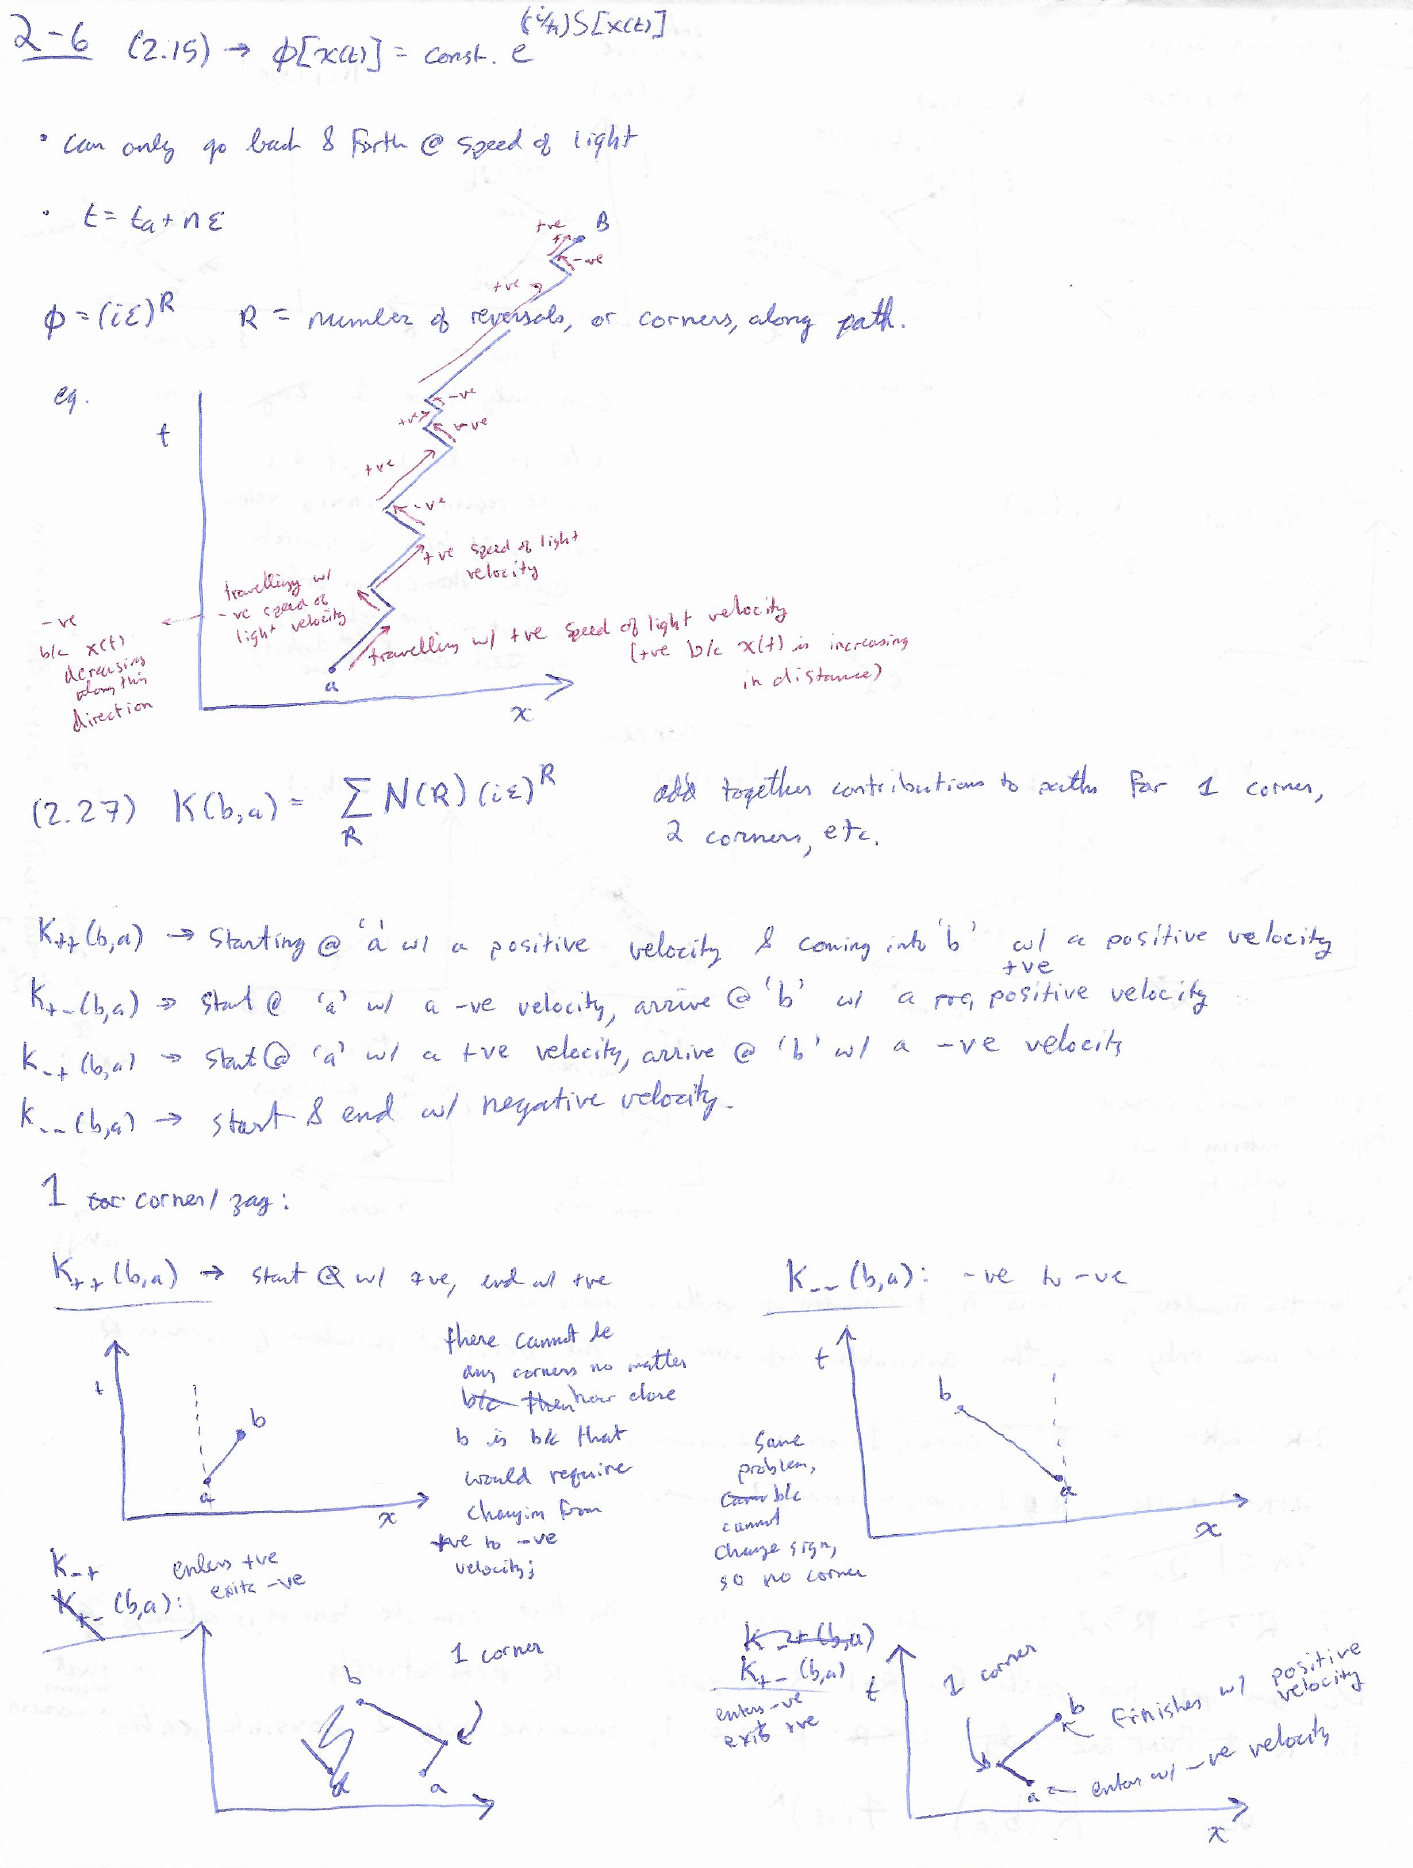
\includegraphics[width=15cm]{FeynmanQ2dash6p1.png}
%\centering
\end{figure}

\begin{figure}[t]
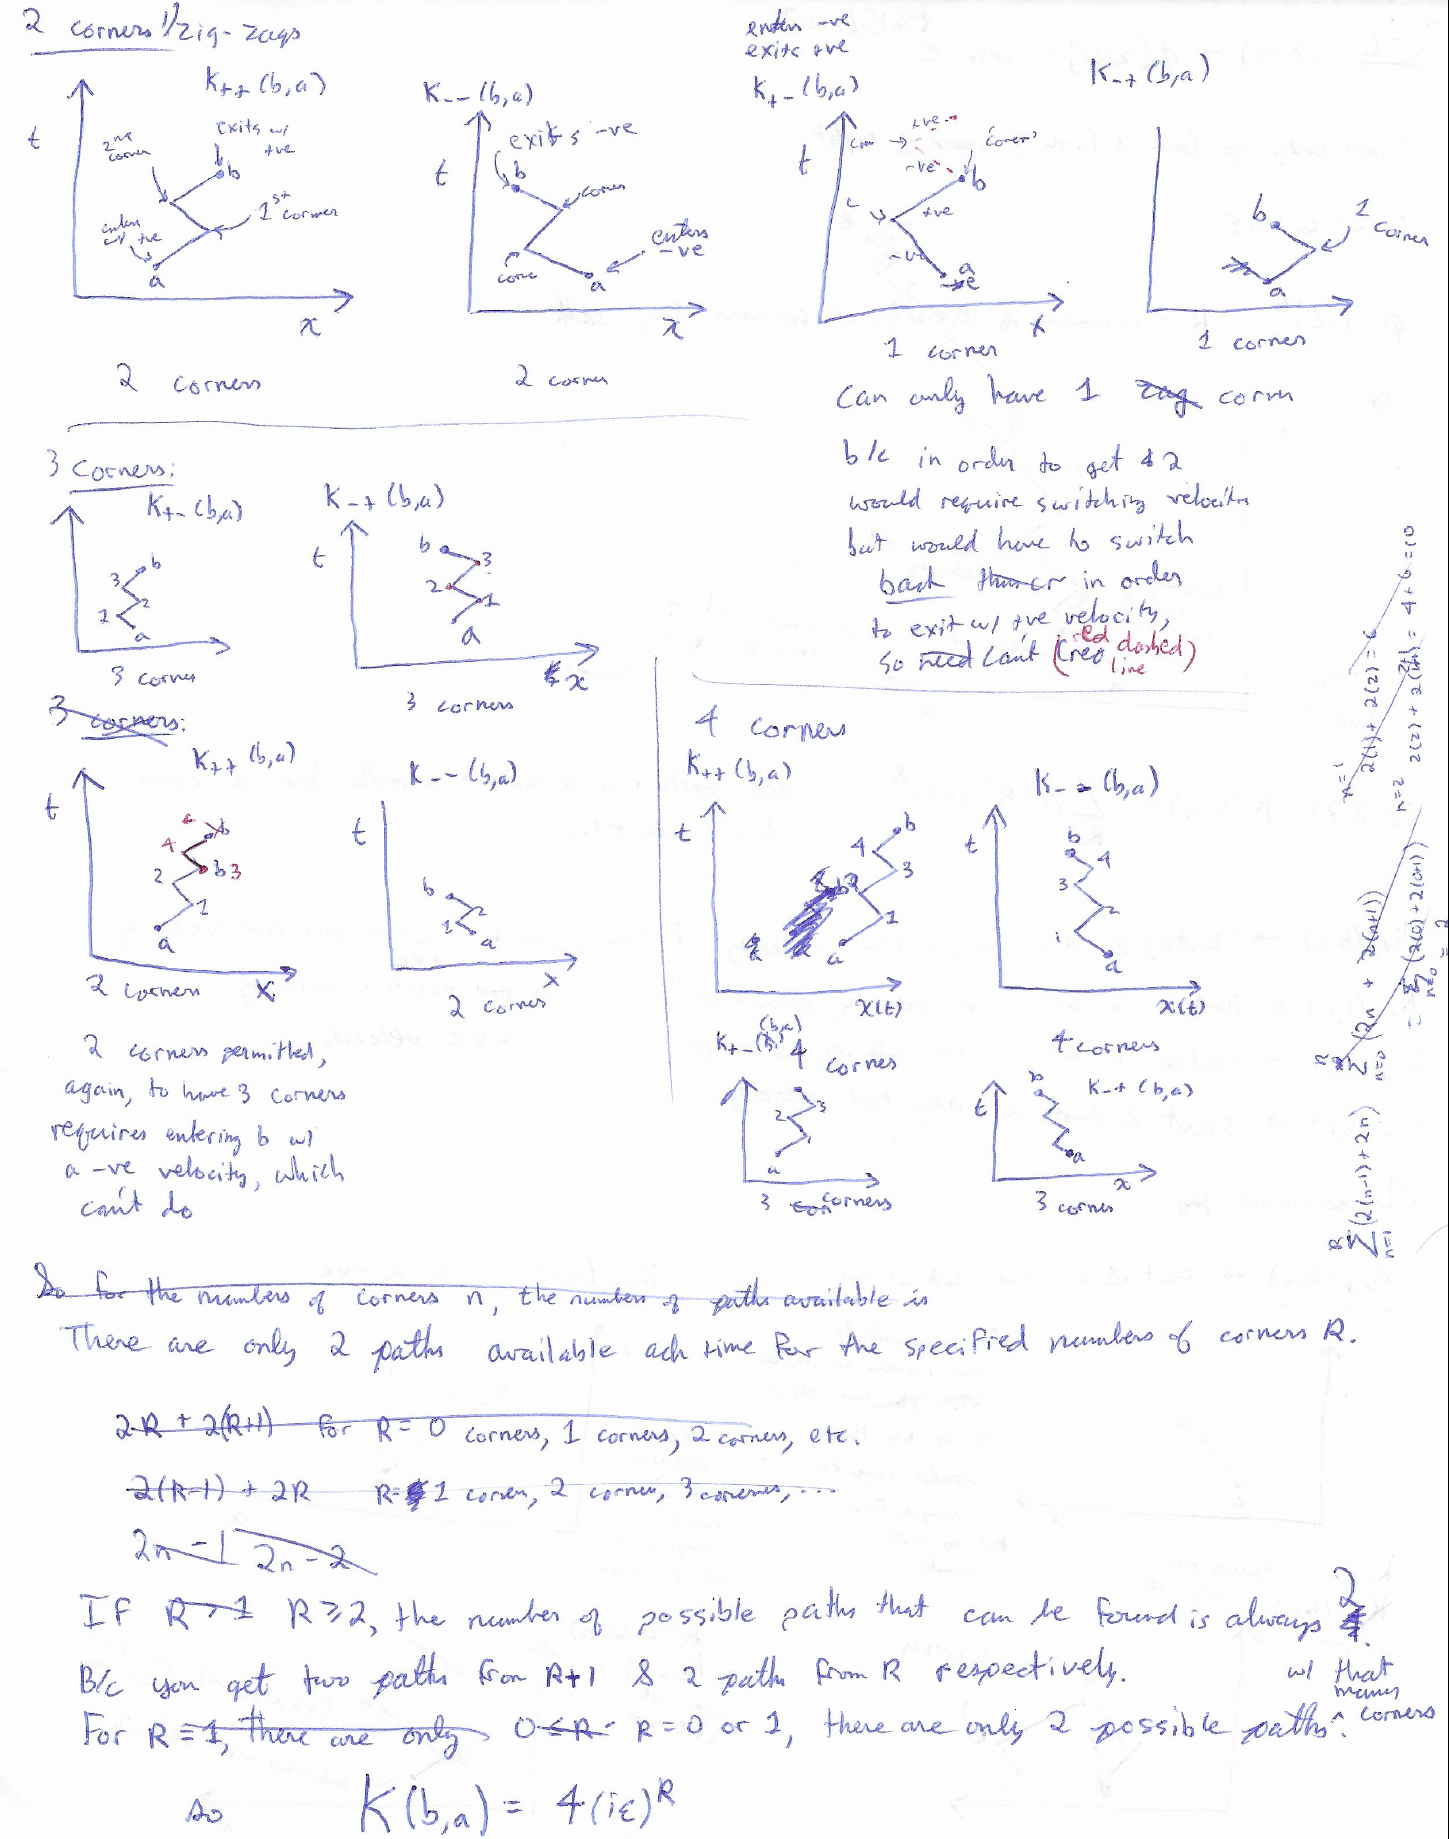
\includegraphics[width=15cm]{FeynmanQ2dash6p2.png}
%\centering
\end{figure}

\begin{figure}[t]
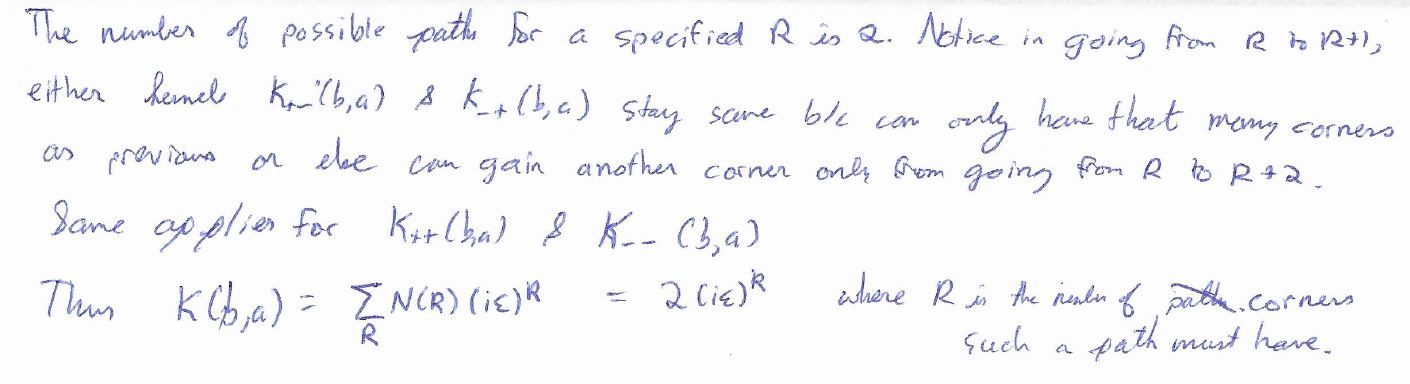
\includegraphics[width=15cm]{FeynmanQ2dash6p3.png}
%\centering
\end{figure}


\section{Conclusion}
``I always thought something was fundamentally wrong with the universe'' \citep{adams1995hitchhiker}

\section{Ya}

\bibliographystyle{plain}
\bibliography{references}
\end{document}
